% !TEX spellcheck = en_US
% Theta min dynamic calculations
%=================================================================================
Since the control region 1.5 has a large wind speed range of \SI{3.28}{m/s} the optimization of the pitch angle could lead to an increase in AEP.
As optimization process a brute force approach was used in order to find the optimum pitch angle for every operating wind speed in region 1.5. 
During the calculation the pitch angle was optimized in a range of \SI{0}{\degree} to \SI{5}{\degree} with a step size of \SI{0.1}{\degree}. 
The results of the optimization can be seen in figure \ref{fig:theta min dynamic}. 
The result shows, that keeping a static pitch angle through region 1.5 is not leading to the optimal power production. 
A calculation of the AEP with a dynamic pitch adjustment for region 1.5 leads to an increase of \SI{0.19}{\%} compared to a static minimum pitch angle of \SI{0.5}{\degree} as shown in section \ref{minimum pitch angle static}.
(Calculated with Weibull parameters of TC III and $k=2$.)
Since the calculation is done without transition regions for the adjustment of the pitch the increase in AEP after implementation of the control behavior is to be expected less than the named \SI{0.19}{\%}.
The approach of changing the pitch angle dynamically in region 1.5 was not implemented in the OPTIMUS Shakti project but could be interesting for further optimization of the developed WT.  

\begin{figure}[h]
	\centering	
	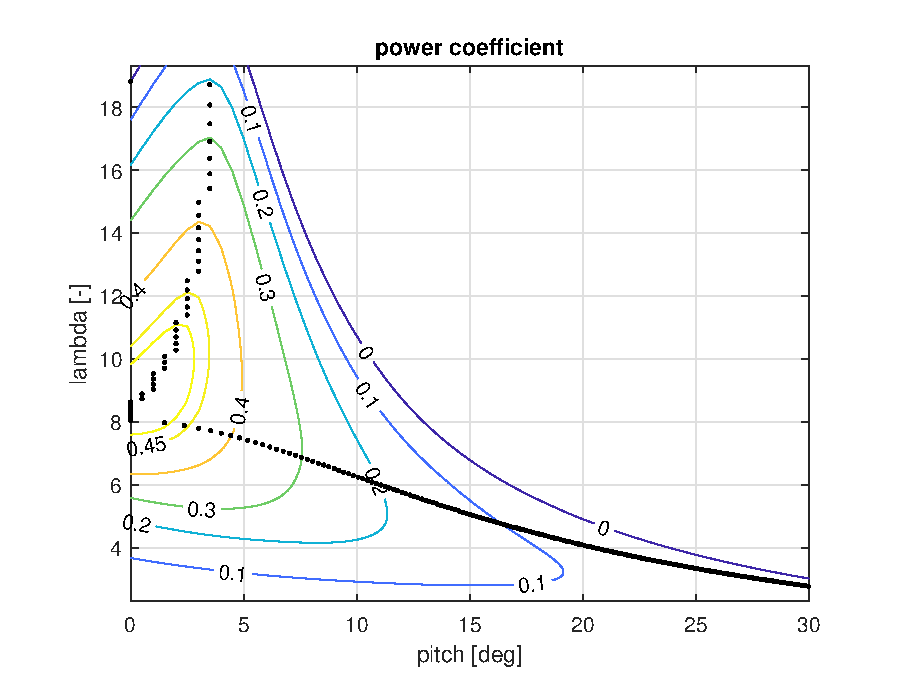
\includegraphics[width=12cm]{Figures/ThetaMinOptDynamic}
	\caption{brute force optimization for minimum pitch angle $\theta$ in region 1.5}
	\label{fig:theta min dynamic}
\end{figure}